% F049: native TikZ/PGFPlots, computed from the stated mathematical model.
\begin{center}
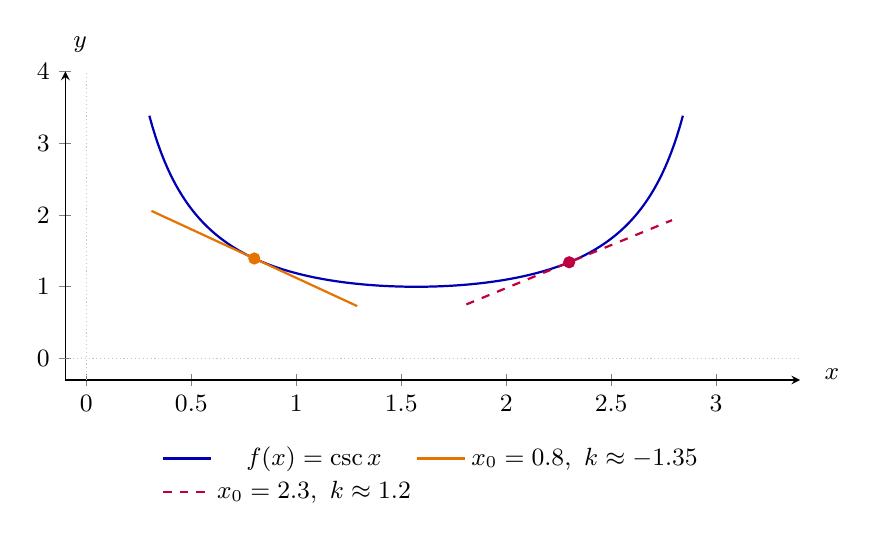
\begin{tikzpicture}[font=\small,>=stealth]
\begin{axis}[width=.90\linewidth,height=5.5cm,xmin=-0.1,xmax=3.4,ymin=-0.3,ymax=4,
axis lines=left,xlabel={$x$},ylabel={$y$},font=\small,
xlabel style={at={(axis description cs:1.02,.02)},anchor=west},
ylabel style={rotate=-90,at={(axis description cs:.02,1.03)},anchor=south},
legend style={at={(axis description cs:.5,-.18)},anchor=north,draw=none,fill=none,font=\small,legend columns=2},
unbounded coords=jump,clip=true,]
\addplot[gray!45,thin,densely dotted,forget plot] coordinates {(-0.1,0) (3.4,0)};
\addplot[gray!45,thin,densely dotted,forget plot] coordinates {(0,-0.3) (0,4)};
\addplot[blue!70!black,thick] coordinates {(0.3,3.3838634) (0.31411996,3.2364595) (0.32823992,3.1019543) (0.34235988,2.978753) (0.35647984,2.8655139) (0.3705998,2.7610994) (0.38471976,2.6645394) (0.39883971,2.5750008) (0.41295967,2.491765) (0.42707963,2.414208) (0.44119959,2.3417861) (0.45531955,2.2740228) (0.46943951,2.2104992) (0.48355947,2.1508453) (0.49767943,2.0947332) (0.51179939,2.0418712) (0.52591935,1.9919988) (0.54003931,1.9448832) (0.55415927,1.9003149) (0.56827922,1.8581057) (0.58239918,1.8180853) (0.59651914,1.7801) (0.6106391,1.7440101) (0.62475906,1.7096885) (0.63887902,1.6770197) (0.65299898,1.6458979) (0.66711894,1.6162265) (0.6812389,1.5879169) (0.69535886,1.5608878) (0.70947882,1.5350645) (0.72359878,1.5103779) (0.73771873,1.4867644) (0.75183869,1.4641654) (0.76595865,1.4425264) (0.78007861,1.421797) (0.79419857,1.4019304) (0.80831853,1.3828834) (0.82243849,1.3646153) (0.83655845,1.3470887) (0.85067841,1.3302684) (0.86479837,1.3141218) (0.87891833,1.2986183) (0.89303829,1.2837292) (0.90715825,1.2694279) (0.9212782,1.2556893) (0.93539816,1.24249) (0.94951812,1.2298079) (0.96363808,1.2176224) (0.97775804,1.2059141) (0.991878,1.1946647) (1.005998,1.1838571) (1.0201179,1.1734751) (1.0342379,1.1635036) (1.0483578,1.1539283) (1.0624778,1.1447356) (1.0765978,1.135913) (1.0907177,1.1274483) (1.1048377,1.1193304) (1.1189576,1.1115486) (1.1330776,1.1040928) (1.1471976,1.0969536) (1.1613175,1.0901221) (1.1754375,1.0835898) (1.1895574,1.0773489) (1.2036774,1.0713919) (1.2177973,1.0657116) (1.2319173,1.0603016) (1.2460373,1.0551555) (1.2601572,1.0502675) (1.2742772,1.045632) (1.2883971,1.041244) (1.3025171,1.0370986) (1.3166371,1.0331912) (1.330757,1.0295177) (1.344877,1.026074) (1.3589969,1.0228565) (1.3731169,1.0198618) (1.3872369,1.0170868) (1.4013568,1.0145286) (1.4154768,1.0121845) (1.4295967,1.0100522) (1.4437167,1.0081293) (1.4578367,1.006414) (1.4719566,1.0049046) (1.4860766,1.0035995) (1.5001965,1.0024974) (1.5143165,1.0015971) (1.5284364,1.0008979) (1.5425564,1.0003989) (1.5566764,1.0000997) (1.5707963,1) (1.5849163,1.0000997) (1.5990362,1.0003989) (1.6131562,1.0008979) (1.6272762,1.0015971) (1.6413961,1.0024974) (1.6555161,1.0035995) (1.669636,1.0049046) (1.683756,1.006414) (1.697876,1.0081293) (1.7119959,1.0100522) (1.7261159,1.0121845) (1.7402358,1.0145286) (1.7543558,1.0170868) (1.7684758,1.0198618) (1.7825957,1.0228565) (1.7967157,1.026074) (1.8108356,1.0295177) (1.8249556,1.0331912) (1.8390756,1.0370986) (1.8531955,1.041244) (1.8673155,1.045632) (1.8814354,1.0502675) (1.8955554,1.0551555) (1.9096753,1.0603016) (1.9237953,1.0657116) (1.9379153,1.0713919) (1.9520352,1.0773489) (1.9661552,1.0835898) (1.9802751,1.0901221) (1.9943951,1.0969536) (2.0085151,1.1040928) (2.022635,1.1115486) (2.036755,1.1193304) (2.0508749,1.1274483) (2.0649949,1.135913) (2.0791149,1.1447356) (2.0932348,1.1539283) (2.1073548,1.1635036) (2.1214747,1.1734751) (2.1355947,1.1838571) (2.1497147,1.1946647) (2.1638346,1.2059141) (2.1779546,1.2176224) (2.1920745,1.2298079) (2.2061945,1.24249) (2.2203144,1.2556893) (2.2344344,1.2694279) (2.2485544,1.2837292) (2.2626743,1.2986183) (2.2767943,1.3141218) (2.2909142,1.3302684) (2.3050342,1.3470887) (2.3191542,1.3646153) (2.3332741,1.3828834) (2.3473941,1.4019304) (2.361514,1.421797) (2.375634,1.4425264) (2.389754,1.4641654) (2.4038739,1.4867644) (2.4179939,1.5103779) (2.4321138,1.5350645) (2.4462338,1.5608878) (2.4603538,1.5879169) (2.4744737,1.6162265) (2.4885937,1.6458979) (2.5027136,1.6770197) (2.5168336,1.7096885) (2.5309536,1.7440101) (2.5450735,1.7801) (2.5591935,1.8180853) (2.5733134,1.8581057) (2.5874334,1.9003149) (2.6015533,1.9448832) (2.6156733,1.9919988) (2.6297933,2.0418712) (2.6439132,2.0947332) (2.6580332,2.1508453) (2.6721531,2.2104992) (2.6862731,2.2740228) (2.7003931,2.3417861) (2.714513,2.414208) (2.728633,2.491765) (2.7427529,2.5750008) (2.7568729,2.6645394) (2.7709929,2.7610994) (2.7851128,2.8655139) (2.7992328,2.978753) (2.8133527,3.1019543) (2.8274727,3.2364595) (2.8415927,3.3838634)};
\addlegendentry{$f(x)=\csc x$}
\addplot[orange!90!black,thick] coordinates {(0.31,2.0574094) (1.29,0.73060625)};
\addlegendentry{$x_0=0.8,\ k\approx-1.35$}
\addplot[only marks,mark=*,orange!90!black,forget plot] coordinates {(0.8,1.3940078)};
\addplot[purple,thick,dashed] coordinates {(1.81,0.75390731) (2.79,1.9281177)};
\addlegendentry{$x_0=2.3,\ k\approx1.2$}
\addplot[only marks,mark=*,purple,forget plot] coordinates {(2.3,1.3410125)};

\end{axis}
\end{tikzpicture}
\par\smallskip{\small $\sin x\ne0$；最低点 $x=\pi/2$ 处斜率为零。}
\end{center}
